\needspace{10\baselineskip}
\begin{center}
\pdfbookmark[1]{10. On Art. 140.}{zusatz-010}
[10. On Art. 140.]
\end{center}
I. Let \(\mathfrak{A},\mathfrak{A}',\mathfrak{A}''\) be the distances of the three points \(A,A',A''\) from the great circle \(BB^*B''\); \(h\) the inclination of this great circle to the ecliptic, and \(H\) the longitude of its ascending node on the ecliptic. We then have
\[
\begin{aligned}
\sin\mathfrak{A}&=\sin h\sin(l-H)\\
\sin\mathfrak{A}'&=\sin h\sin(l'-H)\\
\sin\mathfrak{A}''&=\sin h\sin(l''-H),
\end{aligned}
\]
from which, with the aid of Lemma I in Art. 78, it readily follows that:
\[
\begin{aligned}
1)\quad &\sin\mathfrak{A}\sin(l''-l')+\sin\mathfrak{A}'\sin(l-l'')\\
&\qquad+\sin\mathfrak{A}''\sin(l'-l)=0.
\end{aligned}
\]

II. Let \(B,B^*,B''\) further be the angles which the great circle \(BB^*B''\) makes with \(AB,A'B^*,A''B''\), so that
\[
\begin{aligned}
\sin\mathfrak{A}&=\sin\delta\sin B\\
\sin\mathfrak{A}'&=\sin(\delta'-\sigma)\sin B^*\\
\sin\mathfrak{A}''&=\sin\delta''\sin B''.
\end{aligned}
\]

\SourceLeaf{311}
Equation 1 accordingly takes the following form:
\[
\begin{aligned}
2)\quad &\sin\delta\sin B\sin(l''-l')\\
&\quad+\sin(\delta'-\sigma)\sin B^*\sin(l-l'')\\
&\quad+\sin\delta''\sin B''\sin(l'-l)=0.
\end{aligned}
\]

III. We further have
\[
\left.\begin{aligned}
A''D'-\delta''&=B''D'\\
AD'-\delta&=BD'\\
\frac{\sin B''D'}{\sin BD'}&=\frac{\sin B}{\sin B''}
\end{aligned}\right\}
\quad\text{consequently}\quad a=\frac{R\sin\delta\sin B}{R''\sin\delta''\sin B''}
\]
and
\[
3)\qquad \sin\delta\sin B=\frac{aR''\sin\delta''\sin B''}{R}\mathpunct{\raisebox{.45ex}{,}}
\]
as well as
\[
\left.\begin{aligned}
A''D-\delta''&=B''D\\
A'D-\delta'+\sigma&=B^*D\\
\frac{\sin B''D}{\sin B^*D}&=\frac{\sin B^*}{\sin B''}
\end{aligned}\right\}
\quad\text{consequently}\quad b=\frac{R'\sin\delta'\sin B^*}{R''\sin\delta''\sin B''}
\]
and
\[
4)\qquad \sin B^*=\frac{bR''\sin\delta''\sin B''}{R'\sin\delta'}\mathpunct{\cdot}
\]

Substituting these values from 3, 4 into 2 gives an equation which, on closer examination, is found to be identical with the first equation at the end of Art. 140.

IV. To prove the other formula, let \(P\) be the pole of the ecliptic, \(H\) the point of the ecliptic whose longitude was denoted above by the same letter, thus lying on one great circle with \(BB''\),
\[
\begin{aligned}
\text{thus}\qquad HP&=90^0\\
BP&=90^0-\beta\\
B''P&=90^0-\beta''\\
BHP&=90^0-h\\
BPB''&=\alpha''-\alpha;
\end{aligned}
\]
\begin{center}
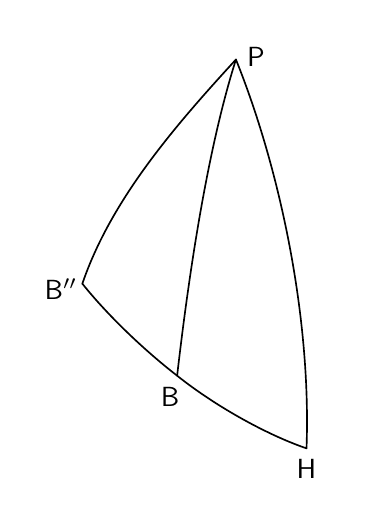
\begin{tikzpicture}[x=.25pt,y=-.25pt,line width=.6pt,line cap=round,line join=round]
\path[use as bounding box] (1850,2220) rectangle (2310,2885);
\draw (2151,2266)..controls(2060,2365)and(1970,2470)..(1929,2590);
\draw (1929,2590)..controls(1965,2635)and(2017,2685)..(2066,2723)..controls(2125,2770)and(2200,2810)..(2253,2828);
\draw (2253,2828)..controls(2260,2640)and(2215,2425)..(2151,2266);
\draw (2151,2266)..controls(2110,2395)and(2083,2575)..(2066,2723);
\node[inner sep=0pt,font=\fontsize{10}{11}\selectfont] at (2180,2262) {\(\mathsf{P}\)};
\node[inner sep=0pt,font=\fontsize{10}{11}\selectfont] at (1898,2598) {\(\mathsf{B}''\)};
\node[inner sep=0pt,font=\fontsize{10}{11}\selectfont] at (2056,2753) {\(\mathsf{B}\)};
\node[inner sep=0pt,font=\fontsize{10}{11}\selectfont] at (2253,2858) {\(\mathsf{H}\)};
\end{tikzpicture}
\end{center}
\[
\sin HB''P=\frac{\cos\beta\sin(\alpha''-\alpha)}{\sin BB''}\quad\text{(in triangle }BPB''\text{)}
\]
\[
\sin HB''P=\frac{\cos h}{\cos\beta''}\quad\text{(in triangle }HB''P\text{),}
\]
consequently
\[
5)\qquad \sin(\alpha''-\alpha)=\frac{\sin BB''\mathbin{.}\cos h}{\cos\beta\cos\beta''}\mathpunct{\cdot}
\]

Now, by Art. 138, (7),
\[
S=\operatorname{tang}\beta\sin(\alpha''-l')-\operatorname{tang}\beta''\sin(\alpha-l'),
\]
\SourceLeaf{312}
hence, since it is readily seen that
\[
\operatorname{tang}\beta=\operatorname{tang}h\sin(\alpha-H),\quad\operatorname{tang}\beta''=\operatorname{tang}h\sin(\alpha''-H):
\]
\[
\begin{aligned}
S=\operatorname{tang}h\{&\sin(\alpha''-l')\sin(\alpha-H)\\
&-\sin(\alpha-l')\sin(\alpha''-H)\}
\end{aligned}
\]
or, since by Lemma I Art. 78 (if \(A,B,C\ldots\ \alpha-l',\alpha''-l',H-l'\) are substituted there, the latter for the former) we have identically
\[
\begin{aligned}
&\sin(\alpha-H)\sin(\alpha''-l')+\sin(H-\alpha'')\sin(\alpha-l')\\
&\qquad+\sin(\alpha''-\alpha)\sin(H-l')=0:
\end{aligned}
\]
\[
S=\operatorname{tang}h\sin(\alpha''-\alpha)\sin(l'-H),
\]
or, substituting the value from 5 for \(\sin(\alpha''-\alpha)\),
\[
6)\qquad S=\frac{\sin h\sin(l'-H)\sin BB''}{\cos\beta\cos\beta''}=\frac{\sin\mathfrak{A}'\sin BB''}{\cos\beta\cos\beta''}\mathpunct{\cdot}
\]

V. We further have
\[
\sin\mathfrak{A}'=\sin AB^*\mathbin{.}\sin B^*=\sin(\delta'-\sigma)\sin B^*.
\]

Thus (end of Art. 140)
\[
U=\frac{S}{\sin(\delta'-\sigma)}=\frac{\sin B^*\sin BB''}{\cos\beta\cos\beta''}
\]
or, since
\[
\sin BB'':\sin BD'=\sin\epsilon':\sin B'',
\]
that is,
\[
\sin BB''=\frac{\sin(AD'-\delta)\sin\epsilon'}{\sin B''}:
\]
\[
U=\frac{\sin(AD'-\delta)\sin\epsilon'\sin B^*}{\cos\beta\cos\beta''\sin B''}
\]
or
\[
\frac{\sin B^*}{\sin B''}=\frac{U\cos\beta\cos\beta''}{\sin(AD'-\delta)\sin\epsilon'}\mathpunct{\cdot}
\]

Substituting this in the above equation \(b=\dfrac{R'\sin\delta'\sin B^*}{R''\sin\delta''\sin B''}\) gives
\[
b=\frac{R'\sin\delta'}{R''\sin\delta''}\cdot\frac{U\cos\beta\cos\beta''}{\sin(AD'-\delta)\sin\epsilon'}\mathpunct{\raisebox{.45ex}{,}}
\]
which is identical with the equation at the end of Art. 140.
\begin{center}\rule{.18\textwidth}{.35pt}\end{center}
